\section{Introduction}
\label{sec:introduction}

Inference-time steering~\cite{wu2025foresight, du2025dynaguidesteeringdiffusionpolices, sun2026latent, kwok2025robomonkey, wang2024inference, hansteer2026, wagenmaker2025steering, yuan2026actasklearnuncertaintyaware} is an emerging way to adapt pre-trained generative robot policies~\cite{chi2024diffusionpolicy, black2024pi_0} at deployment-time and without re-training. 
By treating the frozen policy (e.g., a diffusion policy) as an action proposal generator, inference-time steering focuses on verifying or refining candidate actions before execution. 
Recent work has largely focused on visual verification: candidate actions are rolled out into predicted visual futures (images or latents) and then evaluated with a reward to pick the best action for the task~\cite{wu2025foresight,du2025dynaguidesteeringdiffusionpolices, sun2026latent,yuan2026actasklearnuncertaintyaware}. 
This has proven effective when task success is fully observable by visual cues, like picking the right object or placing it in the right goal.



However, in contact-rich manipulation tasks like pipetting (Fig.~\ref{fig:front_figure}) vision-only steering is insufficient: whether a robot is about to dispense the contents of a pipette mid-transport, or whether its grasp will produce the right force at the goal location, is not observable from wrist or third-person images alone. 
This motivates \textit{multimodal steering}: using vision to guide \textit{which} behavior to pursue, and touch to govern \textit{how} to realize it through contact. 
Yet integrating these two signals during inference-time steering is non-trivial for two key reasons. 
First, visual outcomes and tactile outcomes operate on different time scales: candidate action sequences need to be rolled out long enough to reveal their semantically distinct visual outcomes (e.g., to distinguish which cup the robot is moving towards), whereas tactile outcomes are often local and transient, capturing contact events 
that may be obscured in long-horizon visual predictions (e.g., how much force is applied while squeezing the dropper head). 
Second, even with the perfect outcome predictions, its extremely challenging to have a single unified reward function for verification:
the relative importance of visual and tactile outcomes shifts across task phases, requiring rewards that are themselves phase-conditioned.




To address these challenges, we present
\ours, a visuo-tactile inference-time steering framework for contact-rich manipulation.
Our key idea is a bi-level 
optimization that decomposes multimodal guidance into visual mode selection followed by tactile contact refinement. 
In the visual stage, we perform sampling-and-verification: candidate actions are rolled out with a visuo-tactile latent world model, and a visual verifier selects the sequence that best satisfies the visual objective. In the tactile stage, we treat this selected sequence as an action anchor and apply tactile-guided diffusion editing~\cite{meng2021sdedit} over a short horizon to improve contact execution while remaining close to the visual plan. This decomposition matches each modality with its strength: vision guides the policy toward the intended behavioral mode, while touch refines the physical execution of that mode.

To specify rewards in \ours's bi-level optimization, we use text as a shared task representation to bridge visual and tactile reasoning: the high-level language instruction is decomposed into phase-level visual and tactile objectives, which are then evaluated by semantically-aligned verifiers for each modality.
A visual verifier scores decoded visual predictions for semantic progress, while our text-conditioned tactile verifier scores predicted tactile latents against textual contact objectives. This enables contact-sensitive steering that is \textit{discriminative}, \textit{flexible}, and \textit{efficient}: the verifier can distinguish contacts, adapt to different task phases through language, and guide actions directly in latent space without hand-designing task-specific tactile rewards or decoding tactile predictions.

\para{Statement of Contributions} Our contributions are threefold: (i) we propose a bi-level multimodal guidance framework that uses vision for long-horizon semantic mode selection and touch for targeted contact refinement; (ii) we introduce, to our knowledge, the first language-conditioned tactile reward for robotic manipulation, which scores predicted tactile futures in an aligned latent space, and use it alongside a separate language-conditioned visual reward and a visuo-tactile latent world model for outcome-based policy steering without task-specific reward learning; and (iii) we conduct extensive real-world experiments across three contact-rich manipulation tasks, where \ours improves overall success by $\mathbf{51\%}$ over the base policy, exceeds unimodal steering by at least $\mathbf{33\%}$, and outperforms naive multimodal fusion by at least $\mathbf{20\%}$.


\begin{figure}
    \centering
    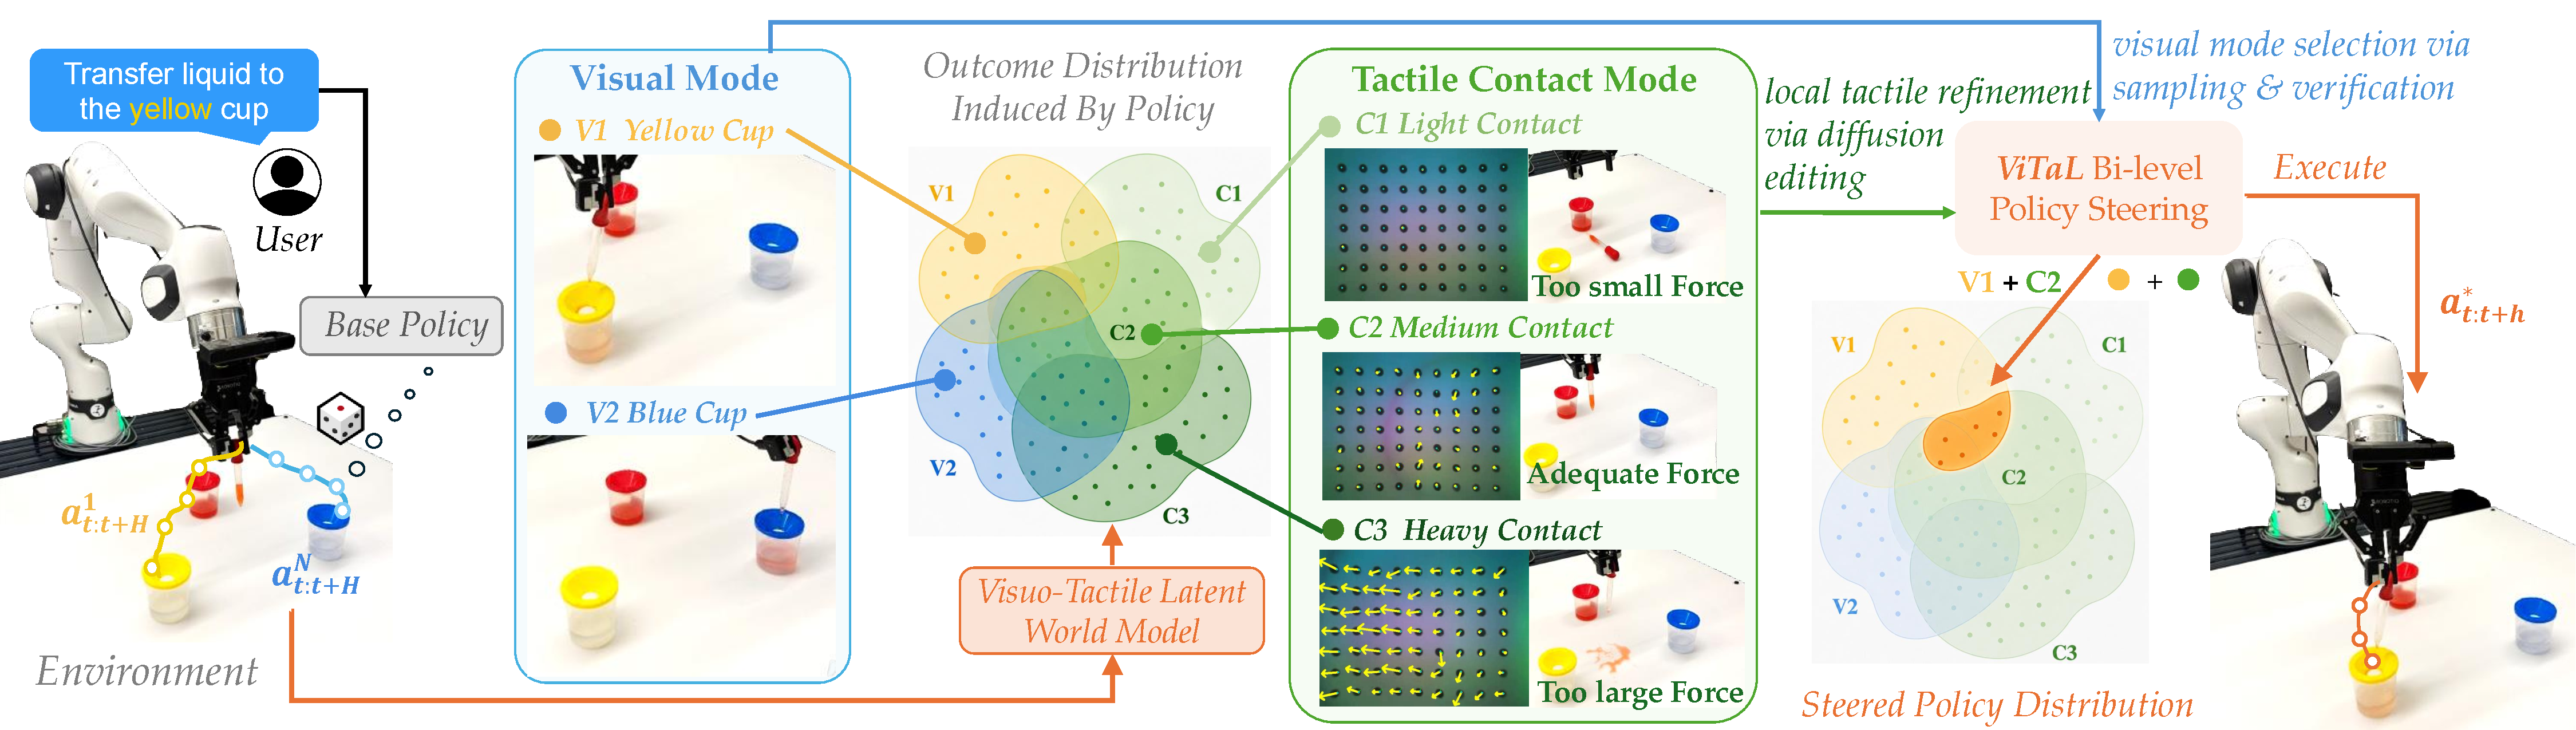
\includegraphics[width=\linewidth]{figures/front_figure_corl_v7.pdf}
    \caption{\textbf{Multi-Modal Policy Steering}. Our method, \ours, selects visual modes and refines local contact, steering the base policy toward actions satisfying both task goals and contact constraints.}
    \vspace{-0.4cm}\label{fig:front_figure}
\end{figure}











